In this chapter, we explore another form of short-ranged interaction, this time induced by spin-spin coupling. For this purpose, we will consider the simplest modification of the spinless case, which is the spin-1 Bose Hubbard model\cite{Tsuchiya_2004}. 
\begin{equation}
    H = -t\sum_{\langle i, j\rangle \sigma} a_{i\sigma}^{\dagger}a_{j\sigma} + \frac{U}{2}\sum_i n_i(n_i - 1) + V_s \sum_i (S_i^2 - 2n_i) - \mu \sum_i n_i
\end{equation}
The spin operators are determined as shown below, using the spin-1 matrices, $\{J_x, J_y, J_z\}$. 
\begin{equation}
    J_x = \frac{1}{\sqrt{2}}
    \begin{pmatrix}
    0 & 1 & 0 \\
    1 & 0 & 1 \\
    0 & 1 & 0
    \end{pmatrix}
    \hspace{0.5cm}
    J_y = \frac{i}{\sqrt{2}}\begin{pmatrix}
    0 & -1 & 0 \\
    1 & 0 & -1 \\
    0 & 1 & 0
    \end{pmatrix}
    \hspace{0.5cm}
    J_z = \begin{pmatrix}
    1 & 0 & 0 \\
    0 & 0 & 0 \\
    0 & 0 & -1
    \end{pmatrix}
\end{equation}
\begin{equation}
    \vec{S_i} = \sum_{\alpha \beta}a_{i\alpha}^{\dagger}\vec{J}_{\alpha \beta}a_{i\beta}
\end{equation}
Note that we have only taken into account the on-site interactions (due to contact scattering and spin-spin coupling). As a result, we do not expect to observe any fundamentally new phases besides the Mott insulator and superfluid. However, now that the bosons have an extra degree of freedom due to their spin ($S = 1, m_s \in \{1, 0, -1\}$), we expect some qualitative differences in the nature of these phases.

\section{Mean Field Theory}
The mean-field decoupling for the spin-1 BHM is is quite similar as for the spinless BHM since we have only introduced additional on-site interaction terms. However, we are now forced to introduce three mean-field parameters for each lattice site, one for each spin projection, $\hat{a}_{i\sigma} = \Psi_{i\sigma} + \delta \hat{a}_{i\sigma}$, where $\sigma \in \{1, 0, -1\}$. This gives us the decomposition of the hopping Hamiltonian as follows.
\begin{align}
    -H_{hop}/zt = \sum_{i\sigma} (\overline{\Psi}_{i\sigma} a_{i\sigma}^{\dagger} + \overline{\Psi}_{i\sigma}^* a_{i\sigma} - \overline{\Psi}_{i\sigma}\Psi_{i\sigma}^*)
\end{align}
As usual, we can assume translational invariance in the ground state and set $\Psi_{i\sigma} = \Psi_{\sigma} \hspace{0.1cm} \forall i$. We will also set $\Psi_{\sigma} \in \mathbb{R}$ for now, but will revisit this assumption further below. The spin-1 BHM can now be written as a sum over single-site Hamiltonians.
\begin{equation}
    H_i\{\Psi_{i\sigma}\} = -zt\sum_{\sigma}(\Psi_{i\sigma} a_{i\sigma}^{\dagger} + \Psi_{i\sigma}^* a_{i\sigma} - \Psi_{i\sigma}\Psi_{i\sigma}^*) + \frac{U_s}{2}(S_i^2 - 2n_i) + \frac{U}{2}n_i(n_i - 1) - \mu n_i
\end{equation}

The spin interaction term can be explicitly computed in terms of the creation/annihilation operators as shown below (where we have introduced the spin index $\overline{1}$ instead of $-1$ for notational clarity).
\begin{equation}
    \begingroup
    \renewcommand*{\arraystretch}{1.5}
    \begin{pmatrix}
        S_x \\
        S_y \\ 
        S_z
    \end{pmatrix}
    \endgroup = 
    \begingroup
    \renewcommand*{\arraystretch}{1.5}
    \begin{pmatrix}
        \frac{1}{\sqrt{2}}(a_{i1}^{\dagger}a_{i0} + a_{i0}^{\dagger}a_{i1} +a_{i\overline{1}}^{\dagger}a_{i0} + a_{i0}^{\dagger}a_{i\overline{1}}) \\ 
        \frac{i}{\sqrt{2}}(-a_{i1}^{\dagger}a_{i0} + a_{i0}^{\dagger}a_{i1} + a_{i\overline{1}}^{\dagger}a_{i0} - a_{i0}^{\dagger}a_{i\overline{1}})\\
        n_{i1} - n_{i\overline{1}}
    \end{pmatrix}
    \endgroup
\end{equation}
\begin{equation}
    S_i^2 = 2n_{i1}n_{i0} + 2n_{i0}n_{i\overline{1}} - 2n_{i1}n_{i\overline{1}} + n_{i1} + 2n_{i0} + n_{i\overline{1}} + n_{i1}^2 + n_{i\overline{1}}^2 + 2a_{i1}^{\dagger}a_{i\overline{1}}^{\dagger}a_{i0}^2 + 2(a_{i0}^{\dagger})^2a_{i1}a_{i\overline{1}}
\end{equation}
Note that most of the terms in the $S_i^2$ operator are block-diagonal in the spin subspaces except for the last two terms which mix the spin components. We can now construct the mean-field Hamiltonian in the occupation basis, $\ket{n_1, n_0, n_{\overline{1}}}$ resulting in the following ansatz for the wavefunction.
\begin{equation}
    \ket{\Psi} = \bigotimes_{i = 1}^M \left (\sum_{n_1, n_0, n_{\overline{1}}} f_{i, n_1, n_0, n_{\overline{1}}} \ket{n_1, n_0, n_{\overline{1}}} \right )
\end{equation}

\subsection{Mott insulator phase}\label{sec:mi_constraint}
When the order parameters satisfy $\Psi_1 = \Psi_0 = \Psi_{\overline{1}} = 0$, the ground state is a Mott insulator. In this section, we will try to understand the nature of the Mott insulator lobes due to the introduction of the spin degree of freedom, by considering the Hamiltonian in the limit $t \ll U$. 
\begin{equation}
    H_i = \frac{U_s}{2}(S_i^2 - 2n_i) + \frac{U}{2}n_i(n_i - 1) - \mu n_i
\end{equation}
The ground state would clearly be a Fock state with a fixed total occupation number, $n_i$ such that it is a superposition of spin states ($\sum_{\sigma}n_{i\sigma} = n_i$). However, note that $S_i^2$, $S_{iz}$ and $n_i$ commute with each other. As a result, a better basis for our analysis is the combined spin basis, $\ket{n_i; S_i, m_i}$ which is defined by the following eigenvalue equations.
\begin{align}
    \hat{S}_i^2 \ket{n_i; S_i, m_i} &= S_i(S_i + 1)\ket{n_i; S_i, m_i} \\  
    \hat{S}_{iz}\ket{n_i; S_i, m_i} &= m_i \ket{n_i; S_i, m_i} \\ 
    \hat{n}_i \ket{n_i; S_i, m_i} &= n_i \ket{n_i; S_i, m_i}
\end{align}
We can then write the ground state energy for the state $\ket{n; S, m}$ as follows.
\begin{equation}
    E(S, n) = \frac{U_s}{2}(S(S+1) - 2n) + \frac{U}{2}n(n+1) - \mu n
\end{equation}
Before we can determine the state $\ket{n;S, m}$, we must discuss the constraints on these quantum numbers. We will loosely follow the arguments presented in Ying (1996)\cite{ying96}. To begin with, we write the form of the spin ladder operators.
\begin{equation}
    S_+ = S_x + iS_y = \sqrt{2}(a_{1}^{\dagger}a_{0} + a_{0}^{\dagger}a_{\overline{1}}) \hspace{1cm} S_- = S_x - iS_y = \sqrt{2}(a_{0}^{\dagger}a_{1} + a_{\overline{1}}^{\dagger}a_{0})
\end{equation}
Since the spin operators obey the $SU(2)$ commutation relations, $[S_{i\alpha}, S_{i\beta}] = i \epsilon_{\alpha\beta\gamma}S_{i\gamma}$, the ladder structure follows and we have $m \in \{0, \pm 1, \pm 2, \dots \pm S\}$, generating $2S+1$ states for a given value of $n$ and $S$. Let us now consider the state $\ket{n;S, -S}$ to determine the allowed values of $S$. Applying $S_z$ on this state gives us the following relations:
\begin{align}
    2n_1 &= (n - S) - n_0 \\
    2n_{\overline{1}} &= (n + S) - n_{0}
\end{align}
This tells us that $S \leq n$ and further, $(n+S)$ and $n_0$ must both either be even or odd. If we assume that they are odd, we can expand the state $\ket{n; S, -S}$ in the following way.
\begin{equation}
    \ket{\Psi} = \ket{n; S, -S} = \sum_{n_0} c_{n_0} \ket{n_0, \frac{n -n_0 +S}{2}, \frac{n - n_0 - S}{2}} = \sum_{n_0} c_{n_0} \ket{\Psi_{n_0}}   
\end{equation}
By construction, we know that $S_-\Psi = 0$. However, note that the first term $S_-\ket{\Psi_1}$ gives rise to a state having $n_0 = 0$ since $S_- \sim a_{\overline{1}}^{\dagger}a_0$. No other term arising from $S_-\Psi_i$ for odd $i\geq 3$ can generate such a state with $n_0 = 0$. Since the overall result must vanish, we conclude that $c_{1} = 0$. Similarly, by considering the subsequent terms, we can argue that $c_{i} = 0 \hspace{0.1cm} \forall i$.  As a result, $S_-\ket{\Psi} = 0 \implies \ket{\Psi} = 0$, but we know that $\ket{n;S, -S} \neq 0$ so $(N+L)$ cannot be odd. Such an argument fails when $n_0$ is even, since we can conclude $c_i = 0 \hspace{0.1cm} \forall  i \geq 2$ but the lowest order term vanishes under annihilation, so $c_0$ can be non-zero. Thus, we have the constraint that $(n+S)$ must be even. This means that if $n$ is even, $S \in \{0, 2, 4, \dots, n\}$ and if $n$ is odd, $S \in \{1, 3, 5, \dots, n\}$. We will see in the subsequent sections that this constraint directly affects the ground state and hence the phase diagram. 



\subsection{Superfluid phase}
To characterize the superfluid phase, we turn our attention to the set of mean-field parameters which can be grouped like so, $\Psi = (\Psi_1, \Psi_0, \Psi_{\overline{1}}) = \sqrt{n_s}(\eta_1, \eta_0, \eta_{\overline{1}})$, where $n_s = |\Psi|$ is the superfluid density and $\vec{\eta}$ is a normalized spinor. Naturally, when $n_s$ does not vanish, we observe a superfluid phase and can understand its magnetic properties using the average spin given by $\langle \vec{S} \rangle = \sum_{\alpha\beta}\eta_{\alpha}^* \vec{J}_{\alpha\beta}\eta_{\beta}$. Writing out the components, we get:
\begin{equation}
    \begingroup
\renewcommand*{\arraystretch}{1.5}
\begin{pmatrix}
    \langle S_x \rangle \\
    \langle S_y \rangle \\ 
    \langle S_z \rangle
\end{pmatrix}
\endgroup = 
\begingroup
\renewcommand*{\arraystretch}{1.5}
\begin{pmatrix}
    \sqrt{2}(\eta_1\eta_0 + \eta_{\overline{1}}\eta_0) \\ 
    0 \\
    \eta_1^2 - \eta_{\overline{1}}^2
\end{pmatrix}
\endgroup
\end{equation}
Notice that the $y$-component of the average spin vanishes. At this point, we must review our assumption that $\Psi_\sigma \in \mathbb{R}$. Generally, this is valid because the BHM is invariant under the $U(1)$ transformation, $a_i \to e^{i\theta}a_i$ and any phase carried by the order parameter, $\Psi$, can be shifted onto the operators. However, in the spin-1 case, we would like to set all three order parameters, $\Psi_{\sigma}$, to be real. 
\vspace{0.5cm}\\
This creates an issue since the BHM is only invariant under \textit{global} gauge transformations, whereas our order parameters might carry different phases for each spin component, resulting in the transformation $a_{i\sigma} \to e^{i\theta_{\sigma}} a_{i\sigma}$. It can be seen that the spin-1 BHM is invariant under such a transformation only if $\theta_1 + \theta_{\overline{1}} - 2\theta_0 = m\pi$ where $m \in \mathbb{Z}$, precisely due to the spin mixing components of $S^2$. We can still set $\Psi_{\sigma} \in \mathbb{R}$ but this manifests in constraining the spin components of the superfluid strictly to the $x-z$ plane. While this means that we have lost generality, the physics of the system still remains the same and we will continue with this assumption for the sake of simplicity.
\vspace{0.5cm}\\
Getting back to the average spin, a nicer quantity to work with is its magnitude squared.
\begin{align}
    |\langle S \rangle|^2 &= 2(\eta_1\eta_0 + \eta_{-1}\eta_0)^2 + (\eta_1^2 - \eta_{-1}^2)^2 \nonumber\\
    &= 2(\eta_1^2 \eta_0^2 + \eta_{-1}^2 \eta_0^2 + 2 \eta_0^2\eta_1\eta_{-1}) + \eta_1^4 + \eta_{-1}^4 - 2\eta_1^2 \eta_{-1}^2 \nonumber\\ 
    &= (1 - \eta_0^2)\eta_0^2 + (1 - (\eta_1^2 + \eta_{-1}^2))(\eta_1^2 + \eta_{-1}^2) + 4z^2\eta_1\eta_{-1} + \eta_1^4 + \eta_{-1}^4 - 2\eta_1^2 \eta_{-1}^2 \nonumber\\
    &= \eta_0^2 - \eta_0^4 + \eta_1^2 + \eta_{-1}^2 - (\eta_1^2 + \eta_{-1}^2)^2 + 4 \eta_0^2\eta_1\eta_{-1} + \eta_1^4 + \eta_{-1}^4 - 2\eta_1^2 \eta_{-1}^2 \nonumber\\
    &= 1 - \eta_0^4 + 4 \eta_0^2\eta_1\eta_{-1} - 4\eta_1^2\eta_{-1}^2 \nonumber\\
    &= (1 - (\eta_0^2 - \eta_1\eta_{-1})^2)
\end{align}
If we define the singlet operator as $\Theta_i = (a_{i0}^2 - 2a_{i1}a_{i\overline{1}})$, we can directly relate its expectation value to the average spin like so $|\langle S\rangle|^2 = 1 - |\langle \Theta \rangle|^2/n_s^2$. In the ground state, based on the sign of $U_s$, the energy is minimized by $|\langle S \rangle|^2 = 0$ or $|\langle S \rangle|^2 = 1$ corresponding to a 'polar' or 'ferro' superfluid respectively\cite{Tsuchiya_2004}.


\section{Results}
\subsection{Ferromagnetic interactions ($U_s < 0$)}
In this case, the energy is minimized when the net spin of the bosons is maximised. As a result, the superfluid is of 'ferro' nature and exhibits average spin $|\langle S \rangle|^2 = 1$. Similarly, in the Mott insulator phase, each site has a net spin of $S = N$, where $N$ is the number of bosons occupying the site in that Mott lobe. This is allowed by the constraint we obtained in Sec. \ref{sec:mi_constraint}. As a result, there is no qualitative difference in the phase boundaries as compared to the spinless case. Note that whenever we mention 'spin', we mean the quantum number $S$ and not the projection $m_s$. As a result, in the absence of an external magnetic field, the system is actually magnetically unordered. We see that the observations discussed here are in agreement with Fig. \ref{fig:ferro}.
%%% FIG %%%
\begin{figure}[!htb]
    \centering
    \begin{subfigure}[b]{0.49\textwidth}  %keep total sum <1 to show in same line
        \centering
        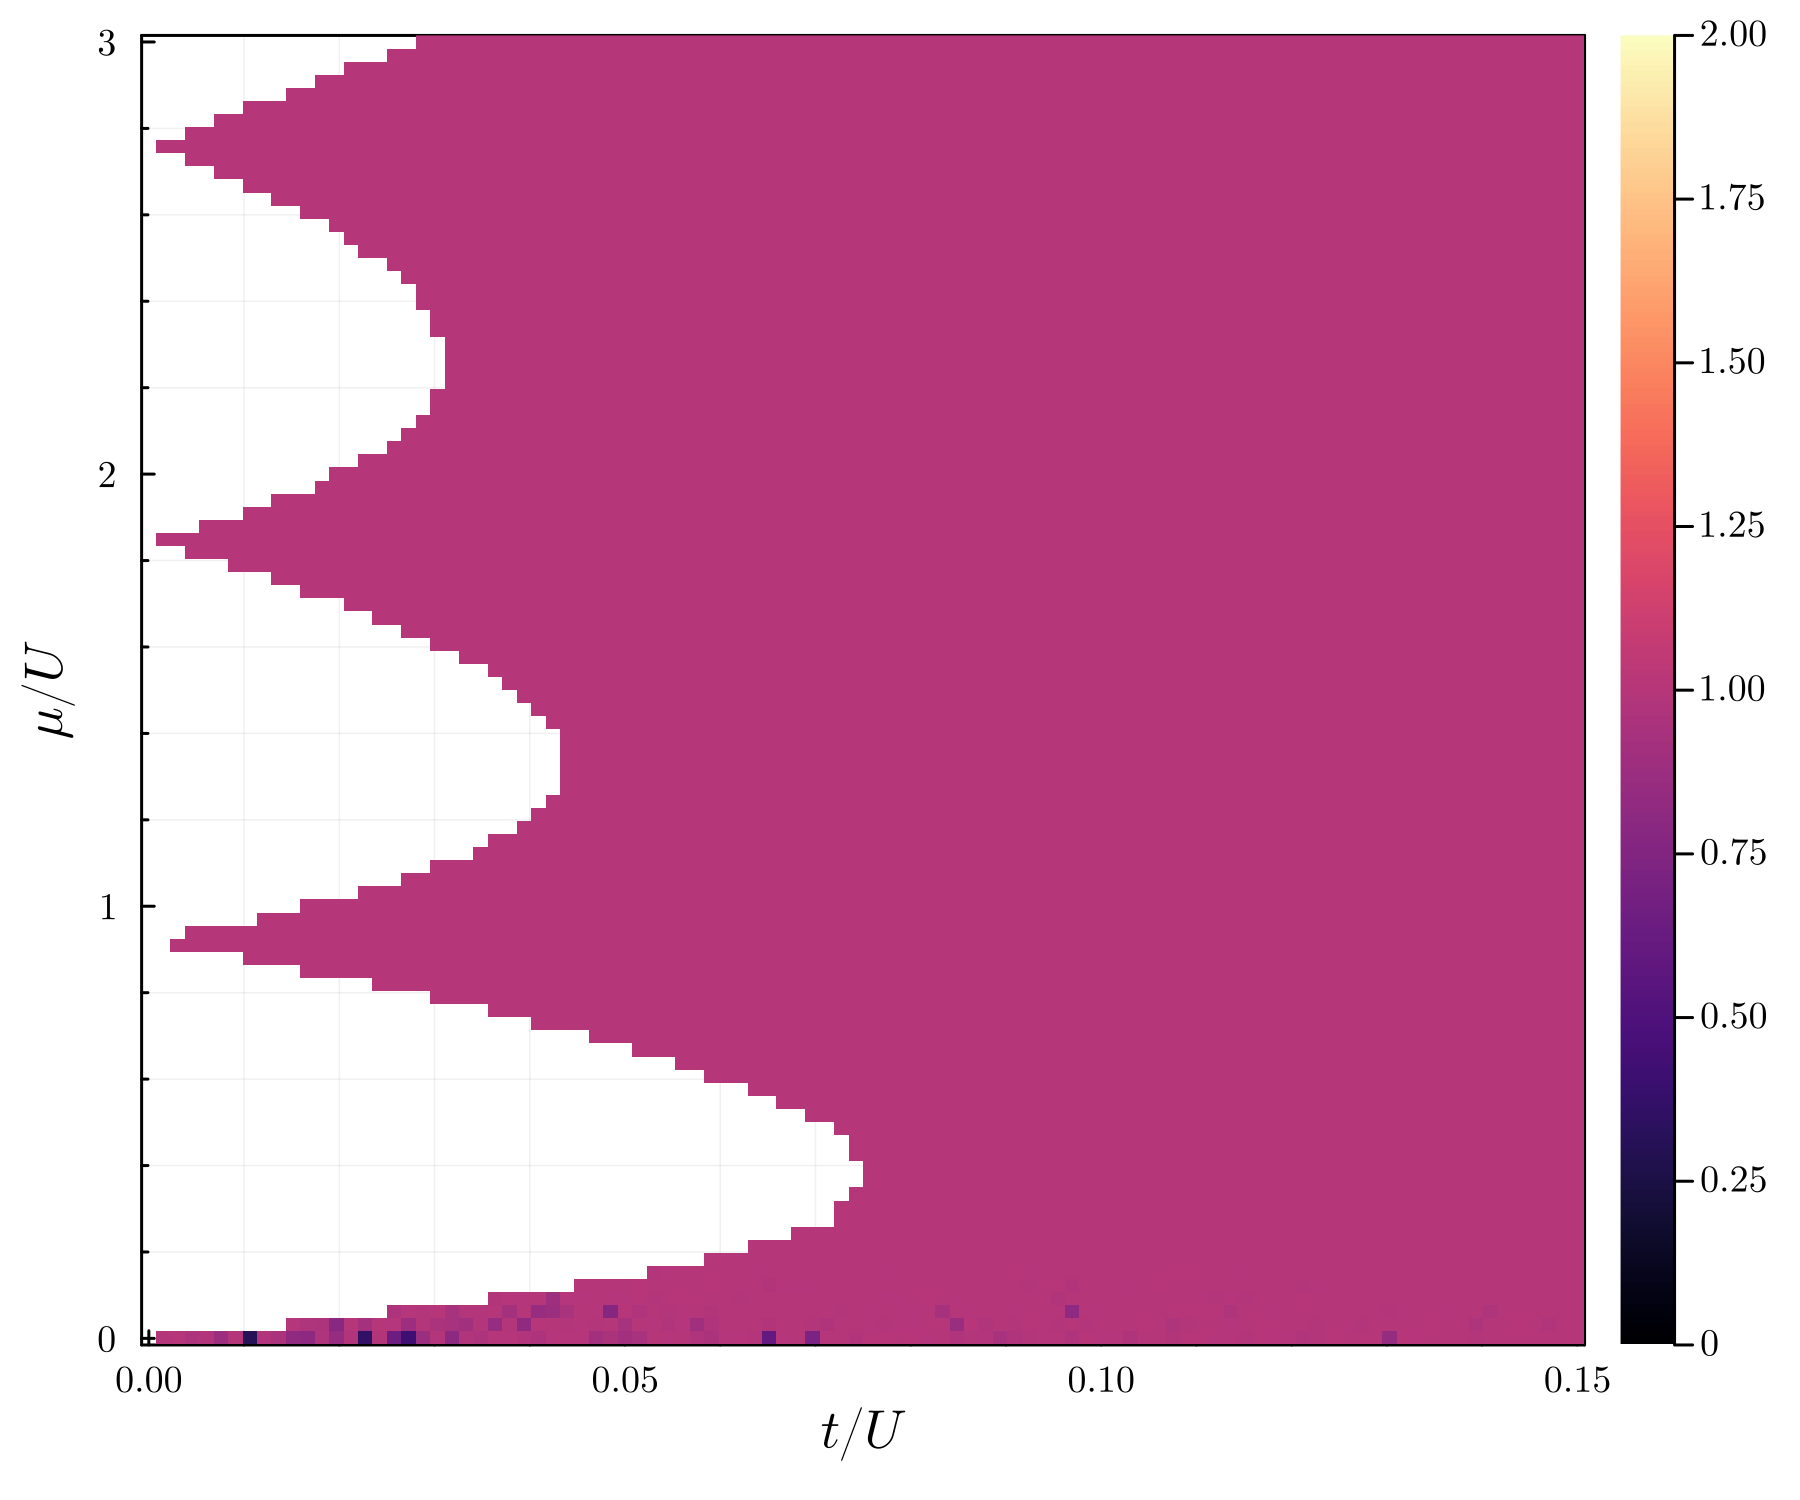
\includegraphics[width=\textwidth]{ch6/ferro_f.png}
        \caption{Average spin, $\langle \mathbf{S} \rangle$}
    \end{subfigure}
    \hspace{1em}  %\hfill
    \begin{subfigure}[b]{0.45\textwidth}
        \centering
        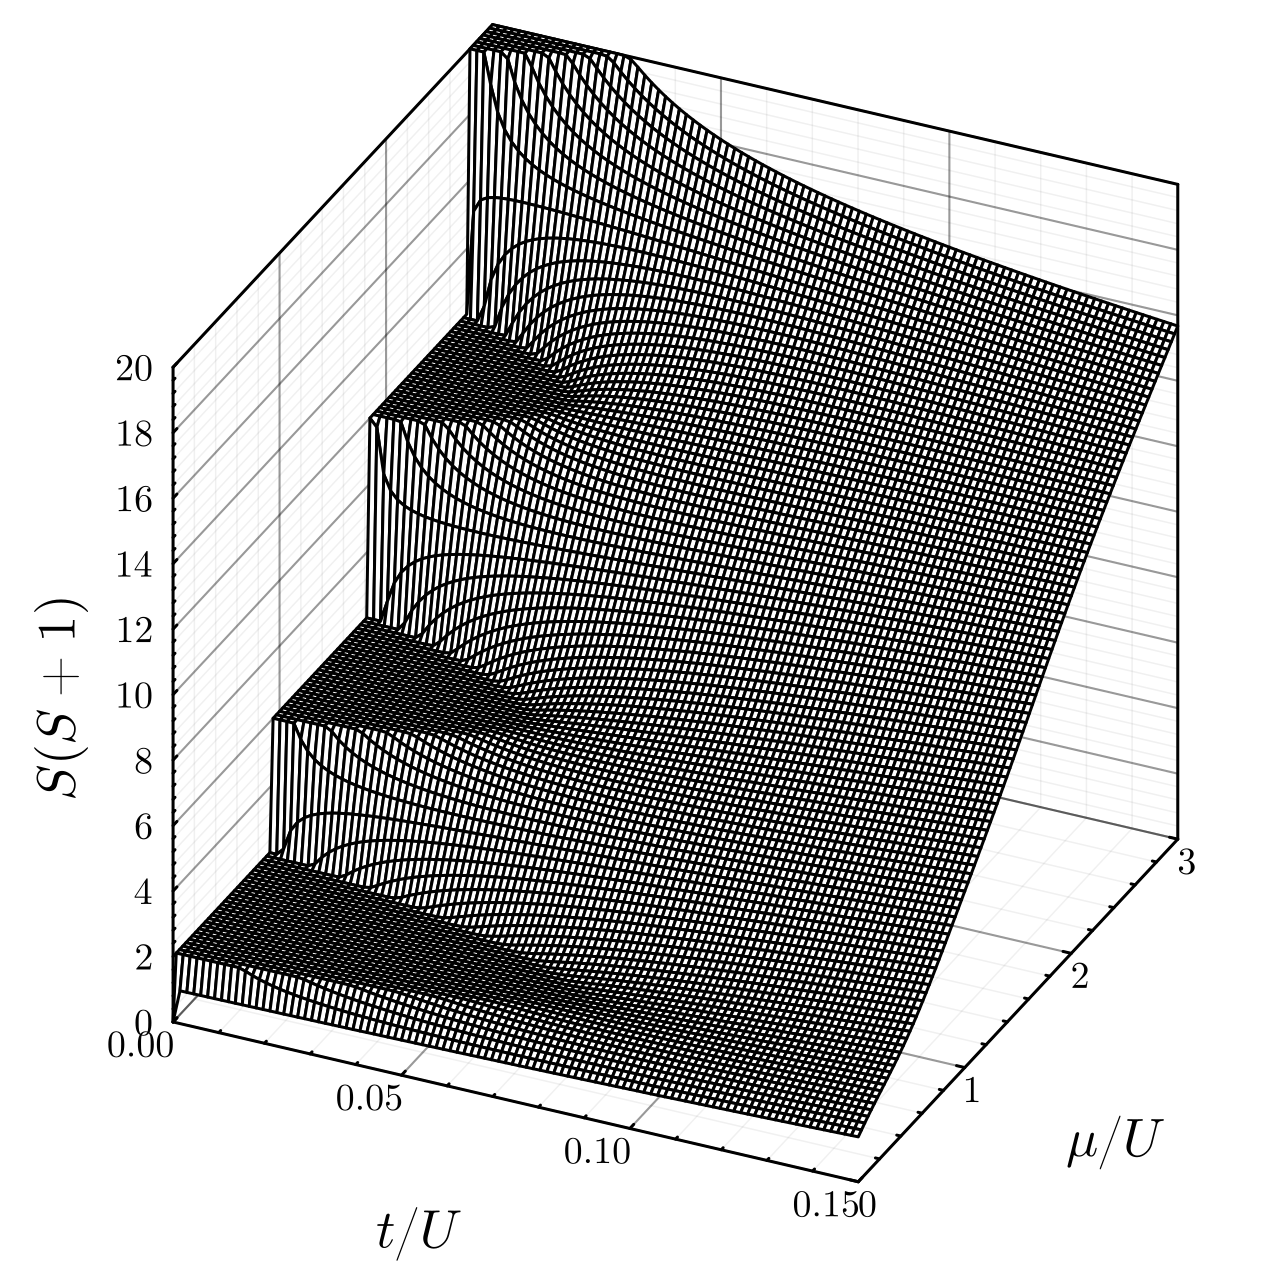
\includegraphics[width=\textwidth]{ch6/ferro_spin.png}
        \caption{Net spin eigenvalue, $\langle S^2 \rangle$}
    \end{subfigure}
    \hspace{1em}
    \vspace{0.5cm}  %\hfill
    \centering
    \begin{subfigure}[b]{0.75\textwidth}  %keep total sum <1 to show in same line
        \centering
        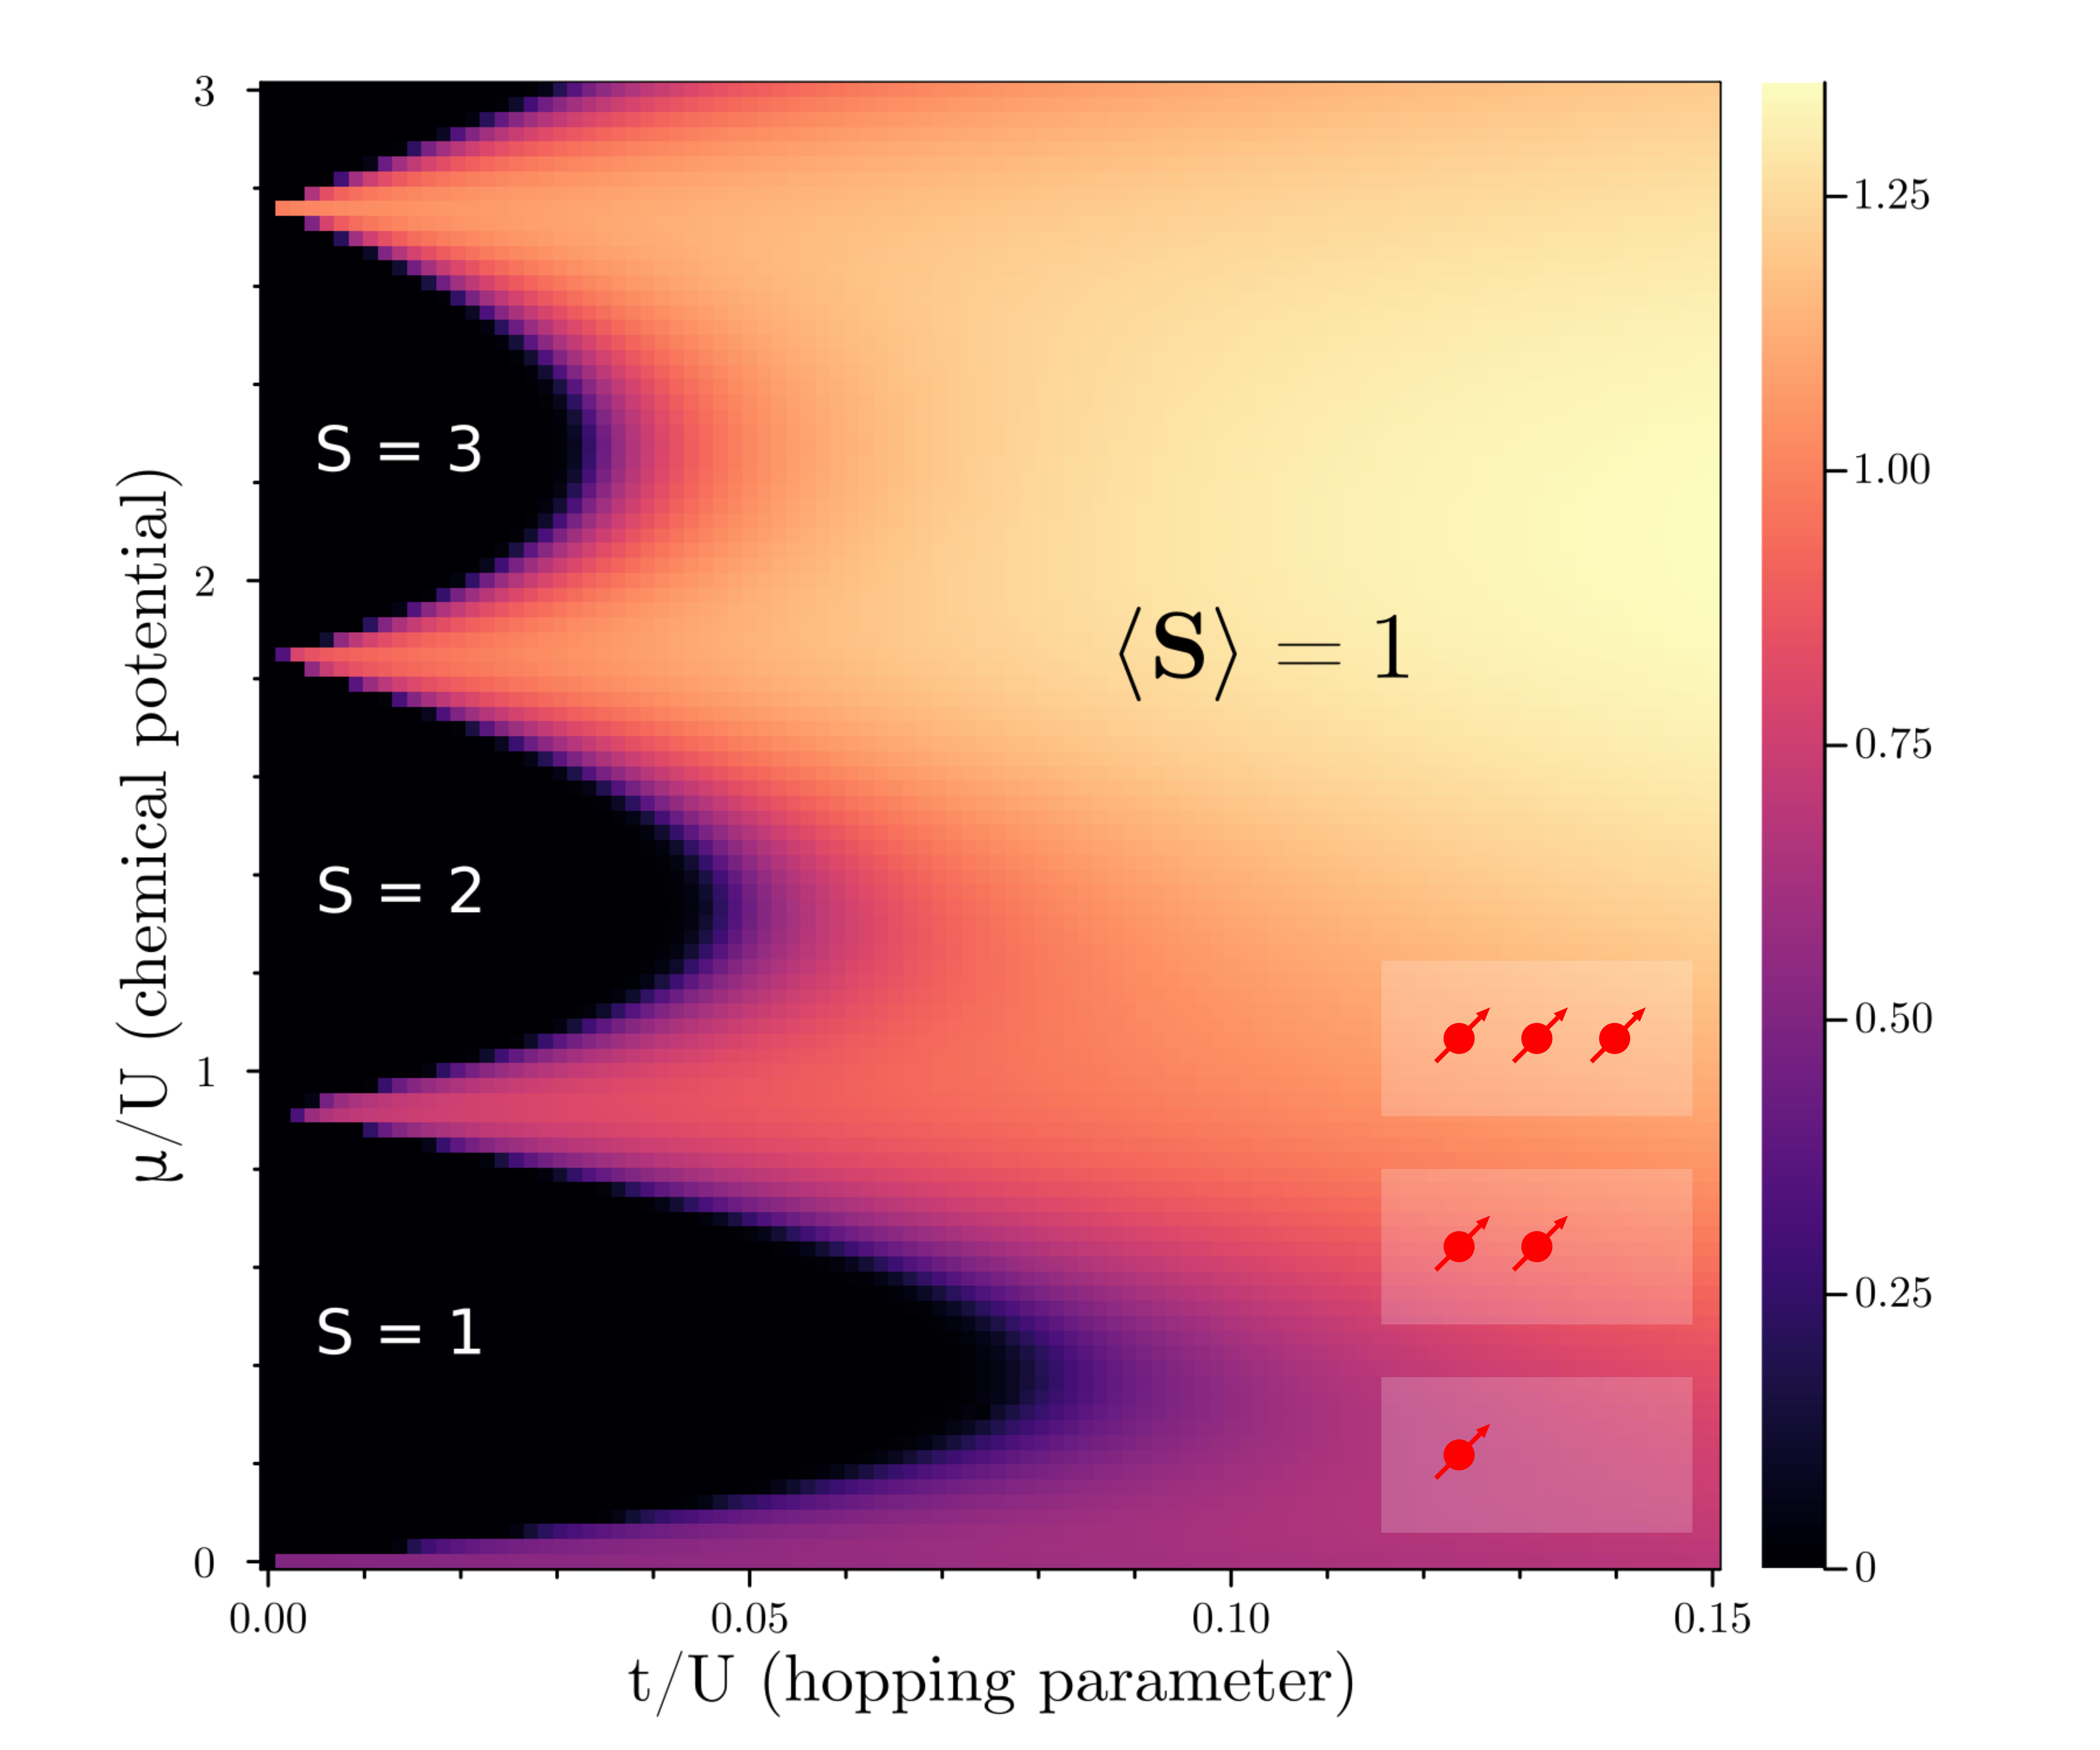
\includegraphics[width=\textwidth]{ch6/ferro_phases.png}
        \caption{Phase diagram}
    \end{subfigure}
    \caption{Ferromagnetic interactions, $U_s = -0.08U$}
    \label{fig:ferro}
\end{figure}
%%% FIG %%%
\FloatBarrier \!\!\!\!\!\!\!\!\!\!\!

\subsection{Anti-ferromagnetic interactions ($U_s > 0$)}

In this case, the energy is minimized when the net spin of the bosons is minimized. As a result, the superfluid is of 'polar' nature and exhibits average spin $|\langle S \rangle|^2 = 0$. Things get interesting in the Mott insulator phase, however, since the constraint from Sec. \ref{sec:mi_constraint} plays a bigger role now as we can see in Fig. \ref{fig:antiferro}. 
\vspace{0.5cm}\\
The Mott lobes with even $N$ is described by the state $\ket{N; 0, 0}$ with $N/2$ pairs of spin singlets, whereas the Mott lobes with odd $N$ is described by the state $\ket{N;1, m}$ such that there is one boson that cannot form a singlet. This has a direct effect on the phase boundaries since singlet formation stabilizes the Mott insulator against the superfluid transition\cite{Tsuchiya_2004}. As a result, there is significant difference in the phase boundary of this system as compared to the spinless case. Further, note that the SF-MI transition is generally second order in nature. However, in this case, only the SF-(odd) MI transitions are second order, while the SF-(even) MI transitions are first order in nature.  

\section{Effective spin-spin interactions}
While the mean-field decoupling allowed us to study the effect of the spin degree of freedom in the ordered phases of the BHM, it also threw away any correlations across the lattice. In the pure Mott insulator limit when $t \ll U$, such a treatment is accurate since the orientations of spins in different lattice sites are genuinely uncorrelated. However, as we introduce finite hopping, the bosons can mediate an interaction between the spins on different sites, thus introducing spin-spin correlations that can give rise to singlet and nematic ordering within the Mott lobes. 
\vspace{0.5cm}\\
In general, one can write an effective spin Hamiltonian for such a case\cite{Tsuchiya_2004}.
\begin{equation}
    H_{\text{eff}} = \sum_{\langle i, j\rangle} (-J_{i, j}^{(0)} - J_{i, j}^{(1)} S_i \cdot S_j - J_{i, j}^{(2)} (S_i \cdot S_j)^2)
\end{equation}
where the coefficients are determined by a perturbative treatment of the hopping term. However, we will not pursue this exercise here since the phenomenon of mediation is complicated by the presence of other terms in the spin-1 BHM. Instead, we study a simpler situation that demonstrates mediation more clearly in the next chapter.   

%%% FIG %%%
\begin{figure}[!htb]
    \centering
    \begin{subfigure}[b]{0.49\textwidth}  %keep total sum <1 to show in same line
        \centering
        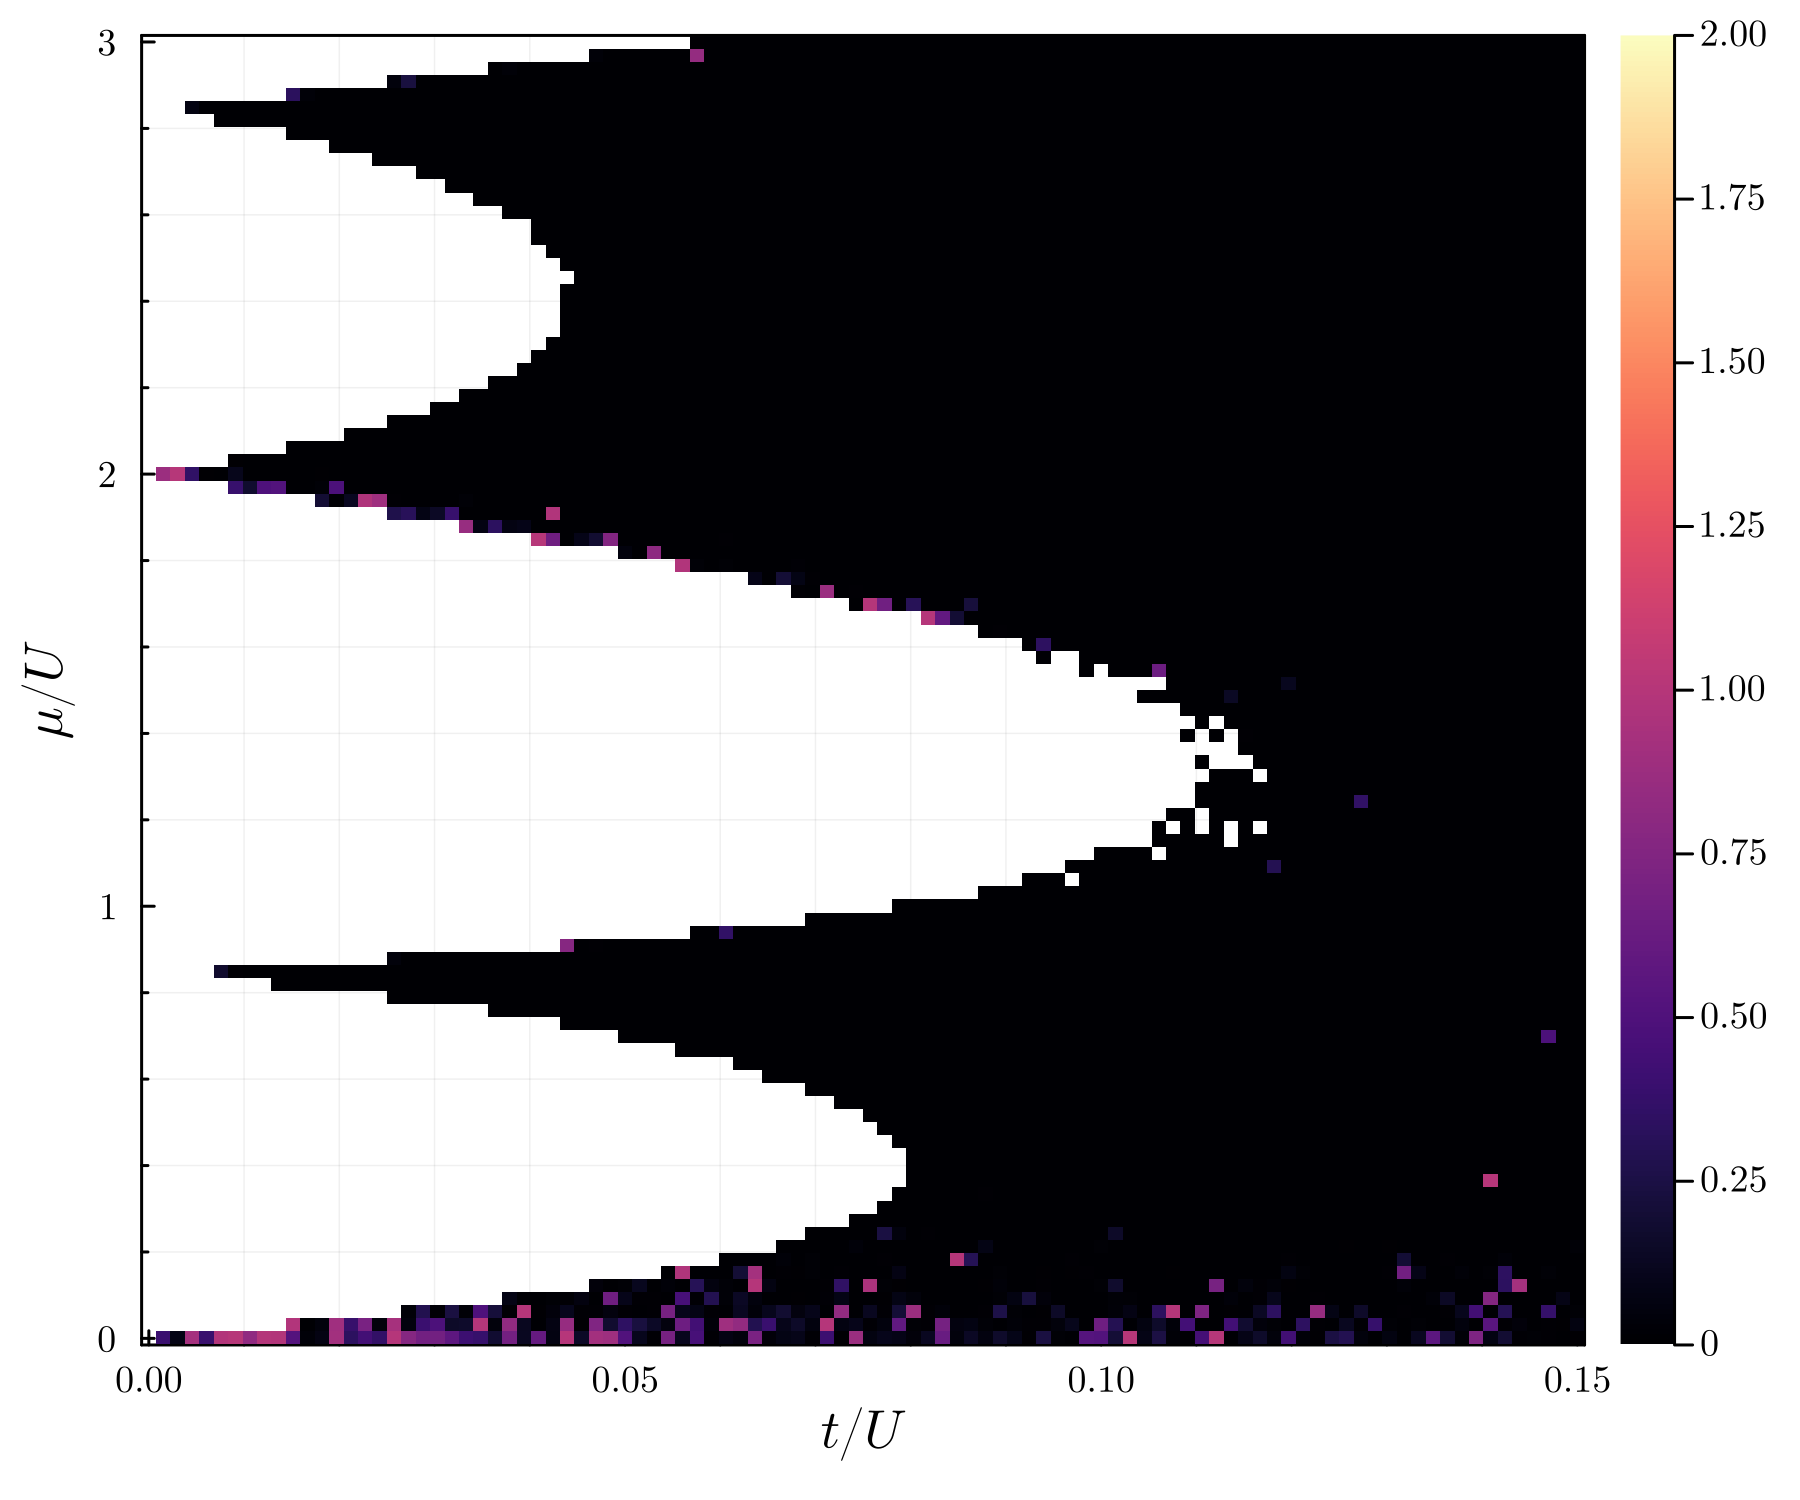
\includegraphics[width=\textwidth]{ch6/antiferro_f.png}
        \caption{Average spin, $\langle \mathbf{S} \rangle$}
    \end{subfigure}
    \hspace{1em}  %\hfill
    \begin{subfigure}[b]{0.45\textwidth}
        \centering
        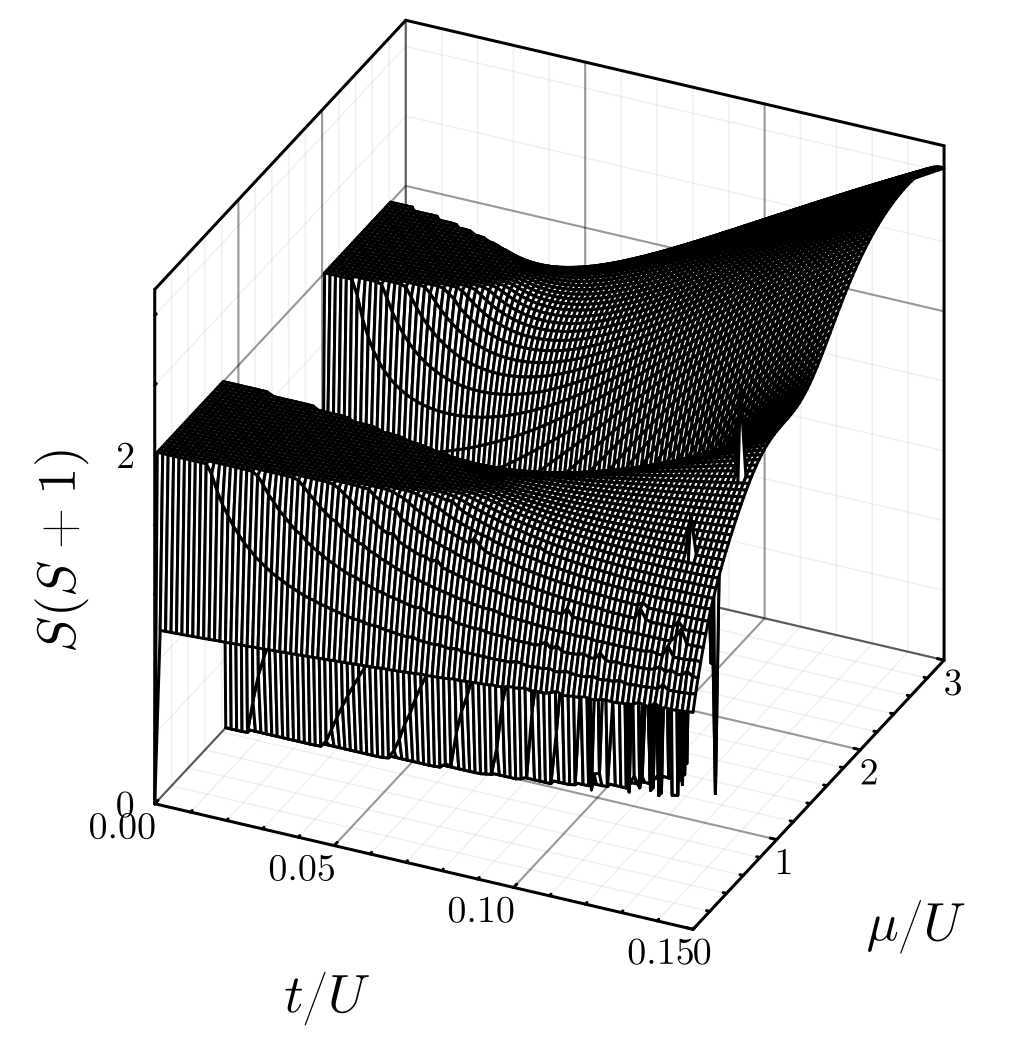
\includegraphics[width=\textwidth]{ch6/antiferro_spin.png}
        \caption{Net spin eigenvalue, $\langle S^2 \rangle$}
    \end{subfigure}
    \hspace{1em}
    \vspace{0.5cm}  %\hfill
    \centering
    \begin{subfigure}[b]{0.75\textwidth}  %keep total sum <1 to show in same line
        \centering
        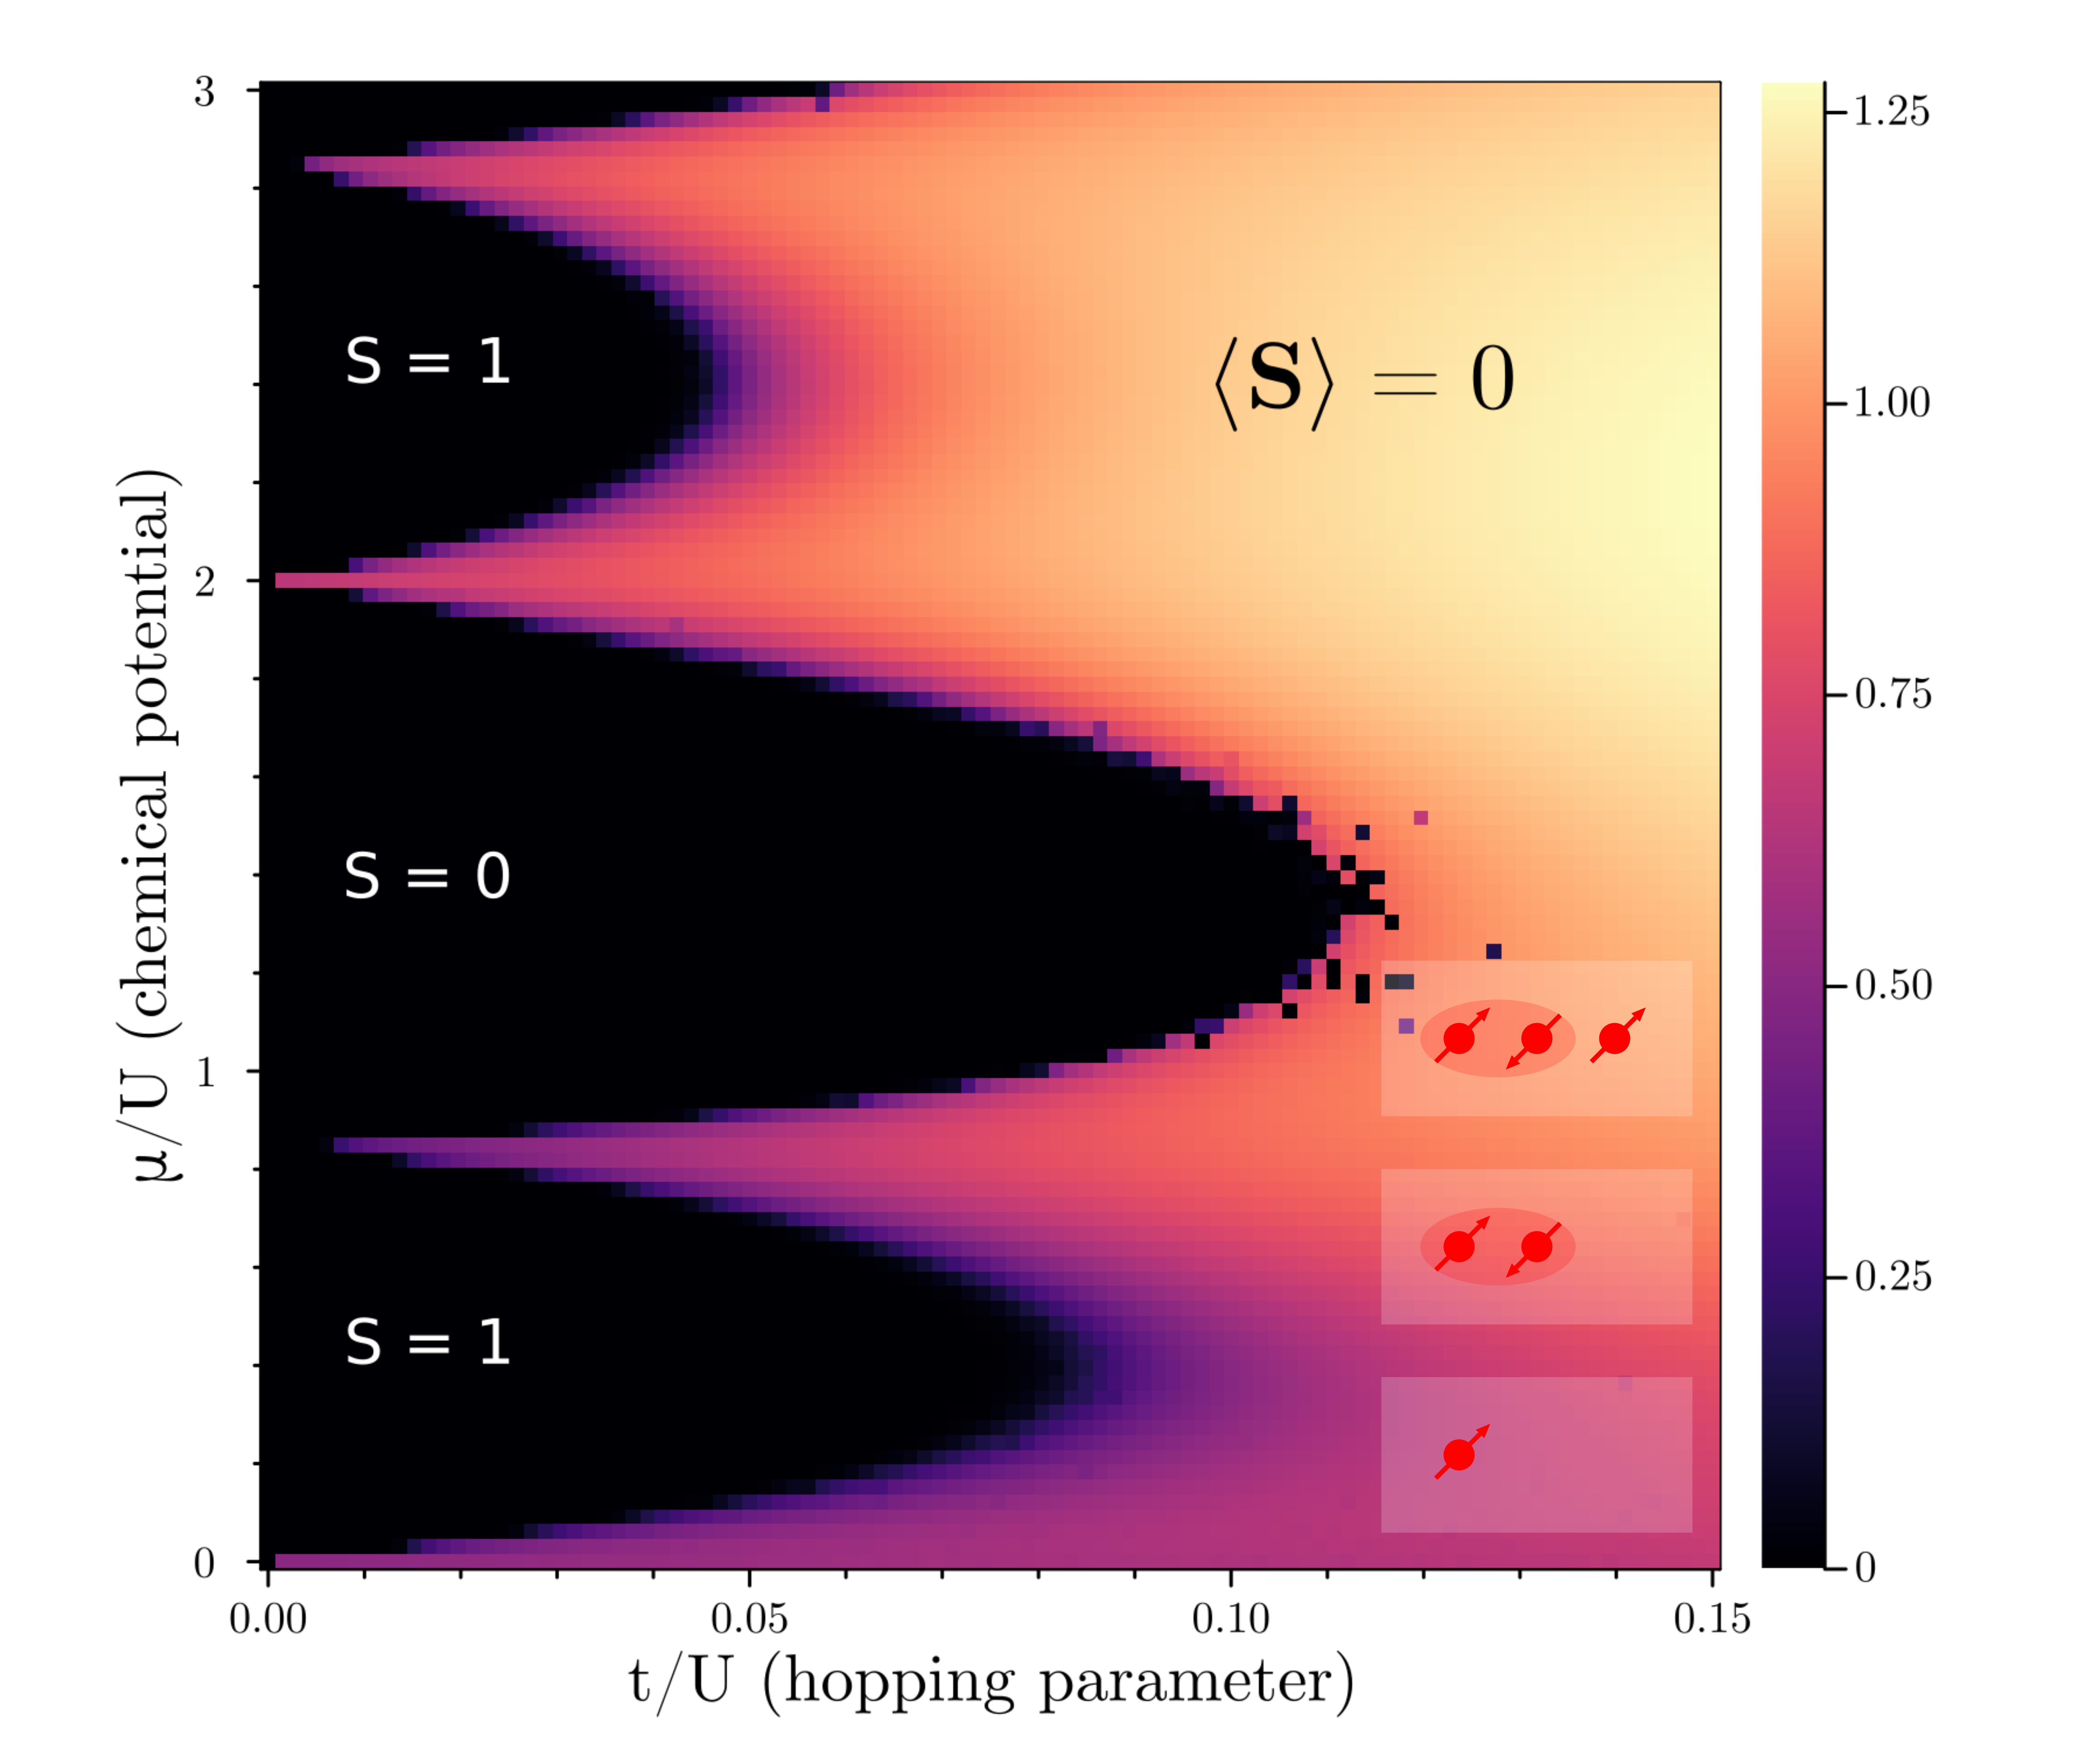
\includegraphics[width=\textwidth]{ch6/antiferro_phases.png}
        \caption{Phase diagram}
    \end{subfigure}
    \caption{Anti-ferromagnetic interaction, $U_s = 0.08U$}
    \label{fig:antiferro}
\end{figure}
%%% FIG %%%
% \FloatBarrier \!\!\!\!\!\!\!\!\!\!\!
